\subsubsection{Postprocessing}

Das Postprocessing stellt einen unverzichtbaren Schritt in der Finite-Elemente-Analyse (FEA) dar. Es ist definiert als der Prozess der Transformation und Aufbereitung der oft hochdetaillierten und komplexen Rohausgaben von FEM-Berechnungen in ein für den Anwender leicht verständliches Format. Im Wesentlichen handelt es sich um die Modifikation oder Verbesserung von Ergebnisdaten, nachdem eine Lösung aus einem Rechenmodell erhalten wurde, mit dem Ziel, aussagekräftige Visualisierungen, Diagramme und andere Ausgaben zu erstellen.

\begin{figure}[!htbp]
\centering
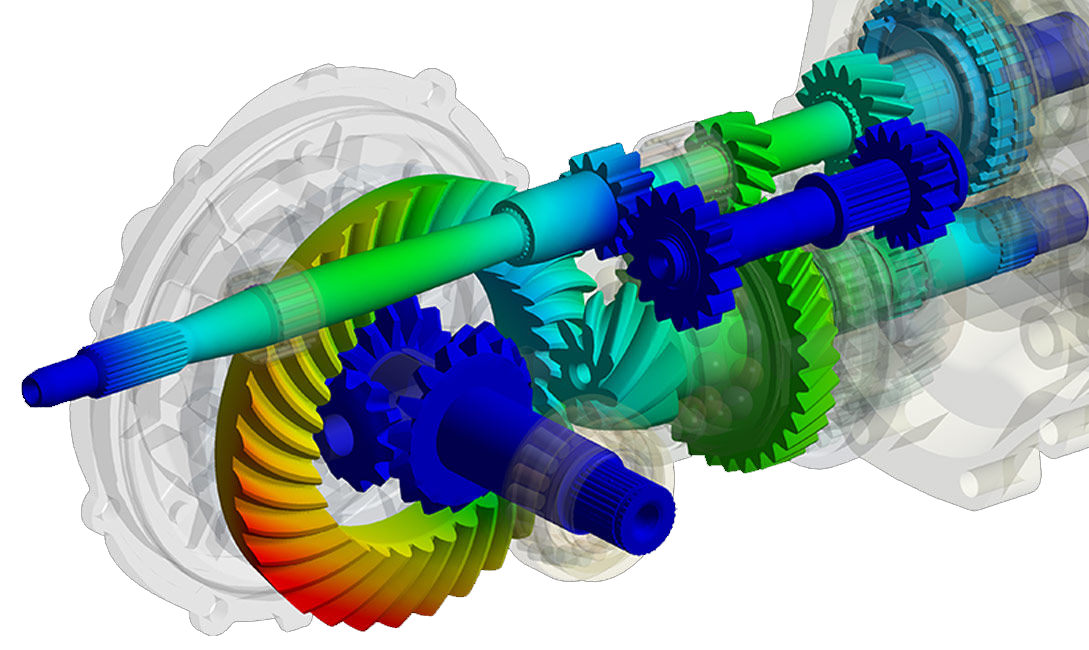
\includegraphics[width=0.625\linewidth]{files/postproc_ansys-7b8042d4d341e019c0ffa102e0eee386.png}
\caption[]{Postprocessing in ANSYS Mechanical nach \href{https://www.padtinc.com/simulation/simulation-product/ansys-mechanical/}{link}.}
\label{postprocansys}
\end{figure}

\paragraph{Postprocessing primärer Grö$\beta$en}

In der Finite-Elemente-Analyse werden die sogenannten primären Grö$\beta$en direkt als Ergebnis der Lösung des globalen Gleichungssystems berechnet. Typische Beispiele hierfür sind Verschiebungen in der Strukturmechanik oder Temperaturen in der Wärmeübertragung. Diese Grö$\beta$en werden explizit an den Knoten des Finite-Elemente-Netzes ermittelt. Die resultierenden Knotenverschiebungen gelten als präzise, da jedem Knoten innerhalb des Netzes ein einziger, eindeutiger Verschiebungswert zugewiesen wird. Dies unterscheidet sich grundlegend von den sekundären Grö$\beta$en, die später erläutert werden.\newline
Die Werte der primären Feldvariablen, die an den diskreten Knoten berechnet werden, dienen dazu, die Werte an allen anderen Punkten innerhalb eines Elements  zu approximieren. Dies geschieht durch Interpolation der Knotenwerte mittels der Formfunktionen des Elementes.
Dies gewährleistet die Inter-Element-Kontinuität der primären Feldvariablen (z.B. Verschiebung oder Temperatur) an den Knotenpunkten. Die Formfunktionen stellen somit die mathematische Brücke dar, die es ermöglicht, die diskrete Lösung an den Knoten in ein kontinuierliches Feld innerhalb jedes Elements zu überführen. Diese Interpolationsfähigkeit ist von grundlegender Bedeutung für die FEM, da sie es erlaubt, mit einer endlichen Anzahl von Freiheitsgraden ein kontinuierliches physikalisches Phänomen anzunähern.

\bigskip\noindent
\begin{tabular}{p{\dimexpr 0.333\linewidth-2\tabcolsep}p{\dimexpr 0.333\linewidth-2\tabcolsep}p{\dimexpr 0.333\linewidth-2\tabcolsep}}
\toprule
Kriterium & Primäre Grö$\beta$en (z.B. Verschiebung, Temperatur) & Sekundäre Grö$\beta$en (z.B. Spannung, Dehnung, Moment) \\
\hline
\textbf{Typ} & Feldvariablen, direkte Lösung & Abgeleitete Grö$\beta$en \\
\textbf{Berechnungspunkt} & Knoten & Gau$\beta$punkte (dann zu Knoten extrapoliert) \\
\textbf{Kontinuität} & C0-kontinuierlich (an Knoten) & Diskontinuierlich an Elementgrenzen \\
\textbf{Genauigkeit (relativ)} & Präzise (eindeutiger Wert pro Knoten) & Weniger präzise (aber genauer an Gau$\beta$punkten) \\
\textbf{Rolle im Postprocessing} & Direkte Ausgabe, Visualisierung & Erfordert Glättung für physikalische Interpretation \\
\bottomrule
\end{tabular}

\bigskip\paragraph{Postprocessing sekundärer Grö$\beta$en}

\begin{figure}[!htbp]
\centering
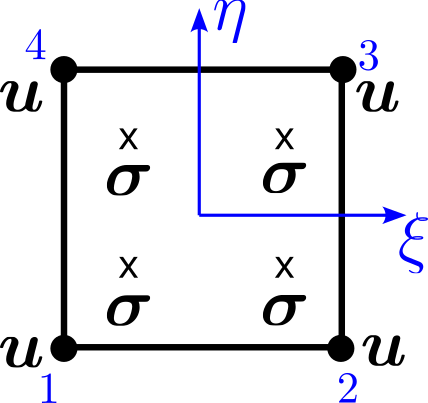
\includegraphics[width=0.375\linewidth]{files/FEM_Postprocessing-c22cc0dbfe91e308fcde8dfd97d168c0.png}
\caption[]{Unterschied zwischen primären und sekundären Grö$\beta$en im Postprocessing.}
\label{postprocFEM}
\end{figure}

Im Gegensatz zu primären Grö$\beta$en werden sekundäre Grö$\beta$en, wie Spannungen, Dehnungen und Momente, nicht direkt an den Knoten berechnet. Stattdessen werden diese abgeleiteten Grö$\beta$en an den sogenannten Gau$\beta$-Integrationspunkten innerhalb jedes Finite-Elements ermittelt.\newline
Der Grund für die Berechnung an Gau$\beta$punkten liegt in der mathematischen Formulierung der FEM, insbesondere im Rahmen der Galerkin-Methode. Die Berechnung von Spannungen und Dehnungen erfolgt aus den Ableitungen der Verschiebungsfelder. Die Gau$\beta$punkte sind die optimalen Punkte für die numerische Integration der Steifigkeitsmatrizen und Lastvektoren und bieten die genauesten Stellen zur Bestimmung dieser abgeleiteten Grö$\beta$en. Der Element-Solver ``kennt'' die Dehnung innerhalb des Elements basierend auf den Knotenverschiebungen und kann daraus die Spannung berechnen. Es ist jedoch wichtig zu verstehen, dass das Element kein ``vollständiges Wissen'' über das Geschehen in seinem Inneren besitzt; es prognostiziert lediglich einige korrekte Antworten an den Gau$\beta$punkten und schätzt bzw. extrapoliert diese wenigen genauen Antworten auf den Rest seiner Fläche.\newline
Um die an den Gau$\beta$punkten berechneten Werte der sekundären Grö$\beta$en an den Knotenpositionen zu erhalten, ist eine Extrapolation dieser Werte von den Gau$\beta$punkten zu den Knoten erforderlich. Diese Extrapolation ist notwendig, da die Knoten oft die primären Punkte für die Ergebnisdarstellung und -interpretation sind.\newline
Es existieren verschiedene Methoden zur Extrapolation von Gau$\beta$punktwerten zu den Knoten, die jeweils unterschiedliche Implikationen für die Ergebnisdarstellung und -genauigkeit haben:

\begin{itemize}
\item \textbf{Zentroidaler Wert (Centroidal Value):} Bei dieser einfachen Methode wird der Durchschnitt der Gau$\beta$punkt-Ergebnisse über alle Gau$\beta$punkte eines Elements berechnet und dieser gemittelte Wert allen Knoten des jeweiligen Elements zugewiesen. Dies führt zu einer sehr starken Glättung der Ergebnisse innerhalb eines Elements.


\item \textbf{Nodalwerte, extrapoliert von Gau$\beta$punkten (Nodal Values Extrapolated from Gauss Points):} Diese Methode verwendet lineare Formfunktionen, um die Gau$\beta$punktwerte zu den Knoten zu extrapolieren. Die Extrapolation entspricht einem Least-Squares-Fit. Sie wird im Allgemeinen für die Mehrheit der linearen Materialmodelle bevorzugt. Eine wichtige Einschränkung ist jedoch, dass diese Option für nichtlineare Materialien unter Umständen nicht gültig ist, da die Extrapolation von Gau$\beta$punktspannungen zu den Knoten zu nodalen Spannungen führen könnte, die die Materialgrenzen überschreiten, was physikalisch inkorrekt wäre.


\item \textbf{Gau$\beta$punktwerte direkt an Knoten platziert (Gauss Point Values Placed at Nodes):} Hierbei wird jedes Gau$\beta$punkt-Ergebnis direkt seinem nächstgelegenen Knoten zugewiesen, ohne weitere Extrapolation. Diese Option ist in der Regel am zuverlässigsten für nichtlineare Materialien, da die direkt zugewiesenen Knotenwerte niemals die Materialgrenzen überschreiten werden.
\end{itemize}

Die grundlegende Natur sekundärer Grö$\beta$en als ``abgeleitete'' Grö$\beta$en hat weitreichende Auswirkungen auf ihre Genauigkeit. Während primäre Grö$\beta$en direkt aus der Lösung der Gleichgewichtsgleichungen resultieren, werden sekundäre Grö$\beta$en durch Rücksubstitution aus den primären Grö$\beta$en berechnet. Da die FEM eine Näherungstechnik ist, propagieren Fehler in den primären Grö$\beta$en und können sich in den abgeleiteten sekundären Grö$\beta$en sogar verstärken, was zu einer höheren Fehleranfälligkeit führt (siehe Konvergenzanalyse der Querkraft bei der Balken-FEM). Die Wahl der Extrapolationsmethode ist somit nicht willkürlich, sondern hängt ma$\beta$geblich vom Materialmodell ab. Eine lineare Extrapolation kann für nichtlineare Materialien physikalisch unmögliche Ergebnisse liefern, was eine konservativere, direkte Zuweisung erforderlich macht. Dies verdeutlicht die Notwendigkeit, das zugrunde liegende Materialverhalten und dessen Wechselwirkung mit den numerischen Methoden genau zu verstehen, da dies die Gültigkeit und den physikalischen Realismus der postprozessierten Ergebnisse direkt beeinflusst.

\bigskip\noindent
\begin{tabular}{p{\dimexpr 0.250\linewidth-2\tabcolsep}p{\dimexpr 0.250\linewidth-2\tabcolsep}p{\dimexpr 0.250\linewidth-2\tabcolsep}p{\dimexpr 0.250\linewidth-2\tabcolsep}}
\toprule
Methode & Prinzip & Anwendungsbereich / Vorteile & Nachteile / Überlegungen \\
\hline
\textbf{Zentroidaler Wert} & Durchschnitt aller Gau$\beta$punktwerte eines Elements wird allen Knoten zugewiesen. & Einfache, schnelle Glättung. & Stark geglättet, verliert lokale Details. \\
\textbf{Nodalwerte, extrapoliert von Gau$\beta$punkten} & Lineare Formfunktionen extrapolieren Gau$\beta$punktwerte zu Knoten. & Bevorzugt für lineare Materialmodelle. & Kann bei nichtlinearen Materialien Materialgrenzen überschreiten. \\
\textbf{Gau$\beta$punktwerte direkt an Knoten platziert} & Jedes Gau$\beta$punkt-Ergebnis wird direkt dem nächstgelegenen Knoten zugewiesen. & Am zuverlässigsten für nichtlineare Materialien, da Materialgrenzen nicht überschritten werden. & Führt zu Diskontinuitäten an Elementgrenzen, da keine Glättung erfolgt. \\
\bottomrule
\end{tabular}

\bigskip\begin{framed}
\textbf{Fragen zum Kapitel}\\
\textbf{Postprocessing}

\begin{itemize}
\item Was sind primäre Grö$\beta$en der FEM in der Strukturmechanik und in der Wärmeleitung?
\item Wo liegen die primären Grö$\beta$en vor?
\item Wo liegen die sekundären Grö$\beta$en bei der FEM vor?
\item Warum werden sekundäre Grö$\beta$en an Gau$\beta$-Integrationspunkten berechnet und nicht direkt an den Knoten?
\item Welche Methoden existieren, um sekundäre Grö$\beta$en von Gau$\beta$punkten zu den Knoten zu extrapolieren?
\item Was ist ein Indikator für eine konvergierte Lösung einer sekundären Grö$\beta$e?
\end{itemize}
\end{framed}